\chapter{Exploratory Investigation}
This thesis project is a continuation of a semester project done in the fall semester of 2016 at NTNU.
The project consisted of a period of development of the experiment framework, followed by a set of experiments.
A report was produced and TODO citation/link to report or paper
This chapter contains a brief summary of the results.
Implementation details of the framework is described in Section \ref{sec:implementation}.


\section{Scope}
The experiments in the previous project concerned the problems of two-dimensional morphogenesis and replication of a set of five "flag" patterns.
This is the same scope as that of \cite{nichele2014evolutionary}, which used an instruction-based encoding and also tested table-based encoding for comparison.
This allowed the results of \cite{nichele2014evolutionary} to act as a benchmark for testing the framework.

TODO make section about morhpogenesis and replication in background instead of explaining here?

\begin{figure*}[h]
\centering
\begin{subfigure}[b]{.20\textwidth}
\centering
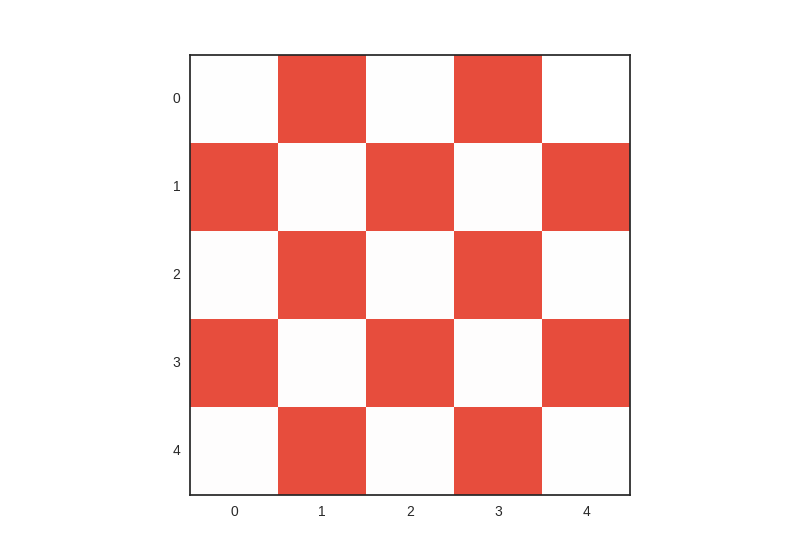
\includegraphics[width=\textwidth]{fig/mosaic}
\caption{5x5 "Mosaic"}
\end{subfigure}%
\begin{subfigure}[b]{.20\textwidth}
\centering
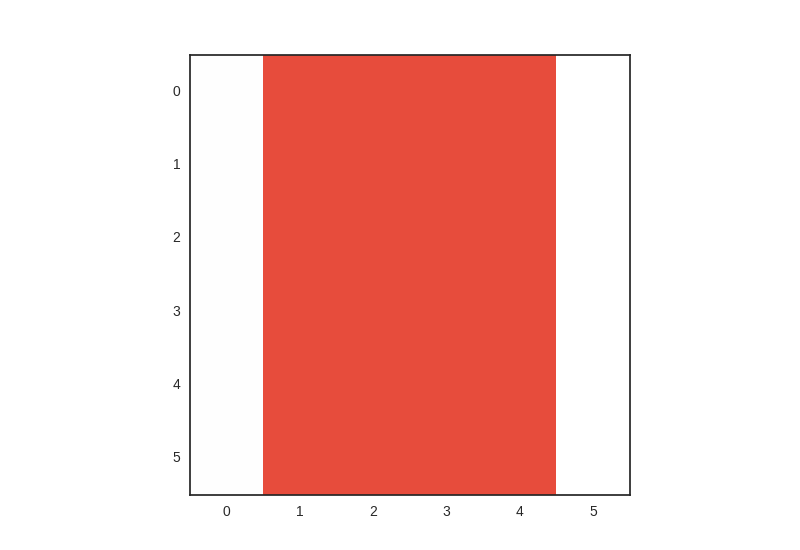
\includegraphics[width=\textwidth]{fig/border}
\caption{6x6 "Border"}
\end{subfigure}%
\begin{subfigure}[b]{.20\textwidth}
\centering
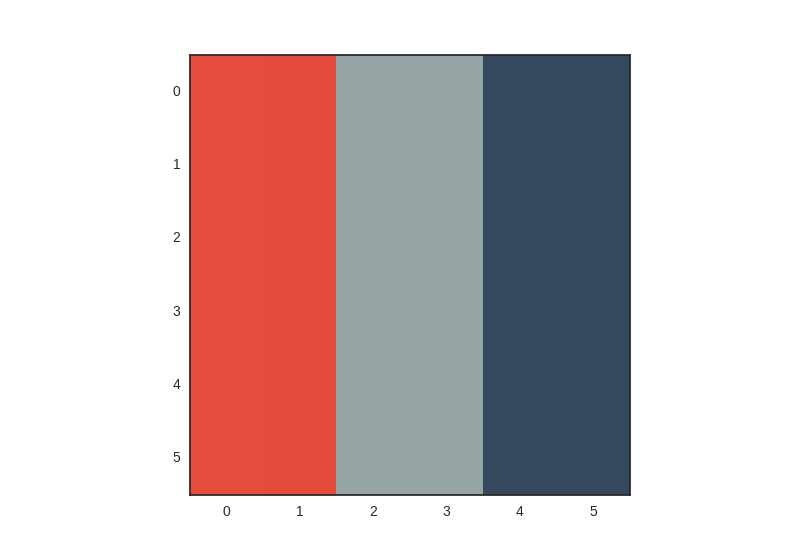
\includegraphics[width=\textwidth]{fig/tricolor}
\caption{6x6 "Tricolor"}
\end{subfigure}%
\begin{subfigure}[b]{.20\textwidth}
\centering
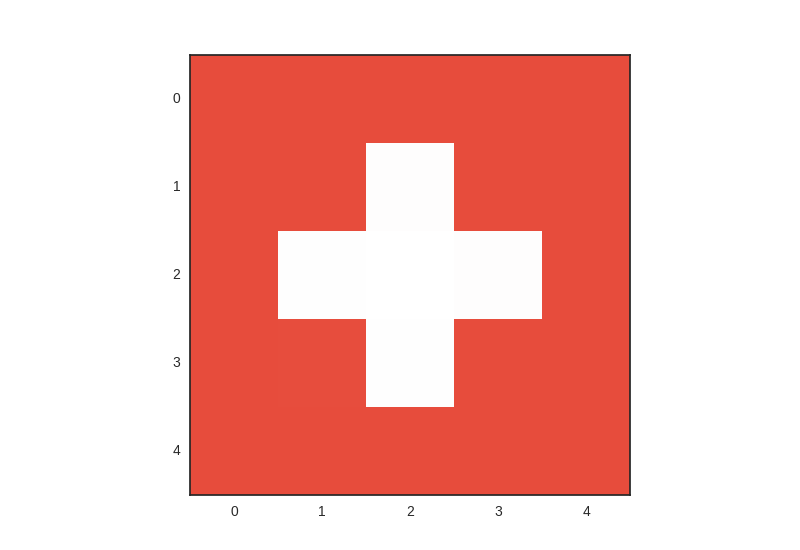
\includegraphics[width=\textwidth]{fig/swiss}
\caption{5x5 "Swiss"}
\end{subfigure}%
\begin{subfigure}[b]{.20\textwidth}
\centering
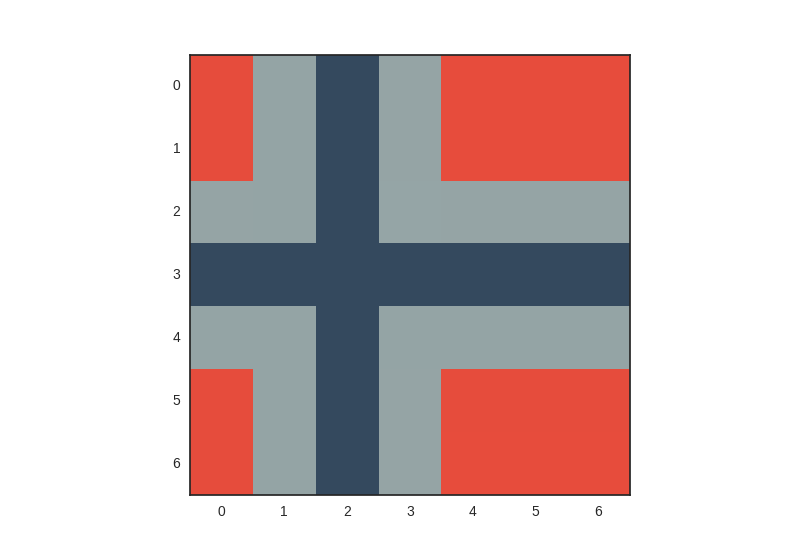
\includegraphics[width=\textwidth]{fig/nordic}
\caption{7x7 "Nordic"}
\end{subfigure}%

\caption{Patterns being investigated.}
\label{fig:patterns}
\end{figure*}

The morphogenesis problem is defined as the development of a complex pattern from a simple "seed" pattern.
The biological analogy and inspiration is \textit{embryonic development},
with the seed pattern also referred to as \textit{zygote}.
Figure \ref{fig:seed} shows the seed patterns used in these experiments.

\begin{figure}[h]
\centering
\begin{subfigure}[b]{.30\columnwidth}
\centering
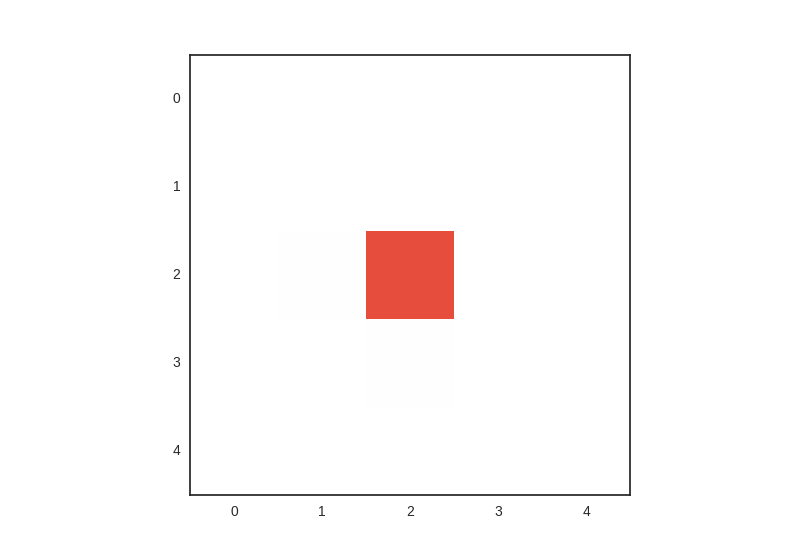
\includegraphics[width=\columnwidth]{fig/seed_5x5}
\caption{5x5}
\end{subfigure}%
\begin{subfigure}[b]{.30\columnwidth}
\centering
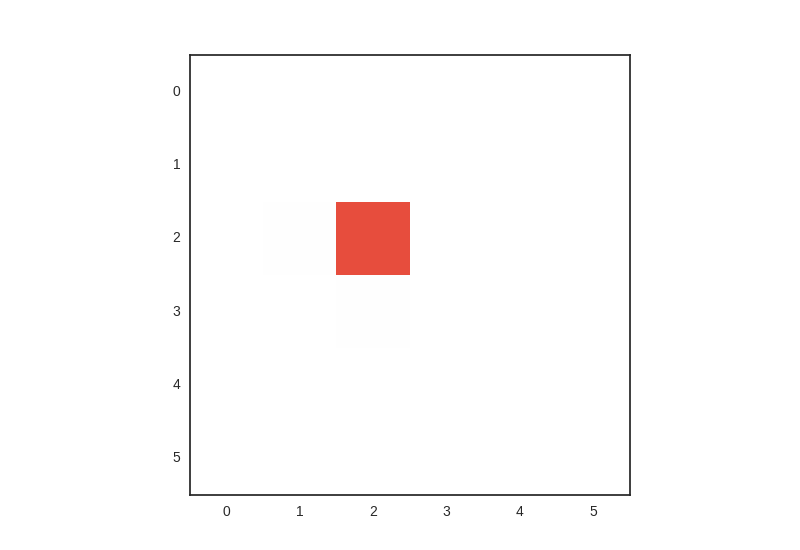
\includegraphics[width=\columnwidth]{fig/seed_6x6}
\caption{6x6}
\end{subfigure}%
\begin{subfigure}[b]{.30\columnwidth}
\centering
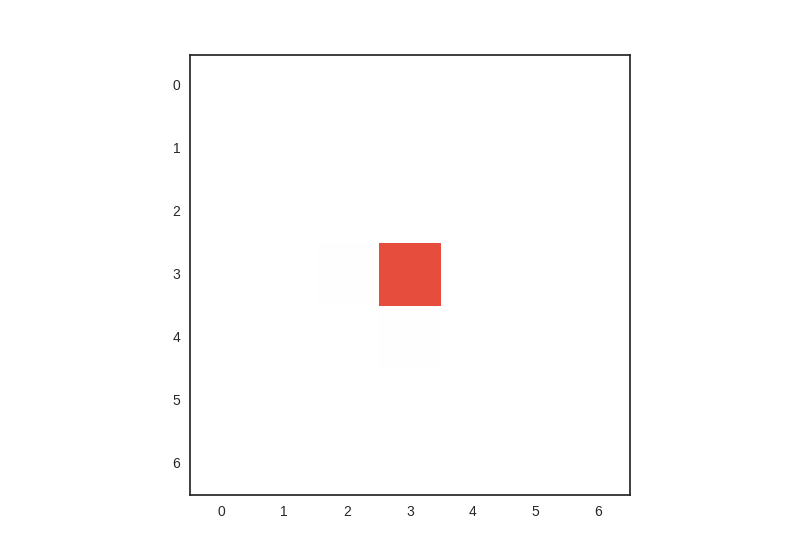
\includegraphics[width=\columnwidth]{fig/seed_7x7}
\caption{7x7}
\end{subfigure}%

\caption{Seed patterns for morphogenesis.}
\label{fig:seed}
\end{figure}

The replication problem start with one instance of some pattern in a larger grid,
and over time develop into a state where multiple copies of the pattern exists in the grid,
which may then replicate again.
The biological analogy of this is cell division and asexual (clonal) reproduction.
For the replication problem the seed pattern is thus one copy of the target pattern in a larger grid.
In these experiments the fitness evalutation function was configuired to require three perfect replicas for a perfect score.
Any additional replicas were not further rewarded.


\section{Results \& Discussion}
The results of the experiments were varied, with some problems being easily solved with CA-NEAT and other problems having few or no solutions found.
Table \ref{tbl:results} summarises the results in terms of success rate and generations of evolution.

\begin{table*}[h]
    \centering
    \caption[Summary of results]{
Summary of results.
The metrics shown are the success rate and the mean number of generations until a solution is found, with standard deviation also shown.
In the case of 100\% success rate, the number of generations column shows how many generations it took until the final solution was found.
In the case of less than 100\% success rate, the column shows how many generations were run until the experiment was stopped.
}
\begin{tabular}{lrrrr}
\hline
 Problem              &   Success rate \% &   Mean gens. &   $\sigma$ gens. &   Gens. until stop \\
\hline
Mosaic morphogenesis      &              100 &                1.2 &                 0.4 &                        2 \\
Border morphogenesis      &                1 &              270   &                 0   &                      509 \\
Tricolor morphogenesis    &              100 &               56.5 &               228.8 &                     2189 \\
Swiss morphogenesis       &               76 &              147.7 &               158.9 &                      600 \\
Mosaic replication        &              100 &                4.2 &                10.6 &                       99 \\
Swiss replication         &              100 &                7.7 &                 5   &                       20 \\
Tricolor replication      &               55 &               55.8 &                52.6 &                      200 \\
Nordic replication        &               0  &                  - &                   - &                      200 \\
\hline
\end{tabular}
\label{tbl:results}
\end{table*}

These results were compared with the results of \cite{nichele2014evolutionary}.
It was found that CA-NEAT was able to significanlty outperform instruction- and table-based encodings at some problems, while also performing much worse at other problems.
TODO more, summarize table

\begin{table}
    \centering
    \caption{TODO}
    \begin{tabular}{llll}
    \hline
    Problem                & Table-based & Instruction-based & CA-NEAT \\ \hline
    Mosaic morphogenesis   & 55\%        & 98\%              & 100\%   \\
    Swiss morphogenesis    & 23\%        & 100\%             & 76\%    \\
    Border morphogenesis   & 69\%        & 98\%              & 1\%     \\
    Tricolor morphogenesis & 19\%        & 46\%              & 100\%   \\
    Mosaic replication     & 85\%        & 100\%             & 100\%   \\
    Swiss replication      & 1\%         & 100\%             & 100\%   \\
    Tricolor replication   & 8\%         & 100\%             & 45\%    \\
    Nordic replication     & 0\%         & 100\%             & 0\%     \\ \hline
    \end{tabular}
\end{table}


Figures \ref{fig:tricolor_point_attractor} and \ref{fig:mosaic7} shows visualizations of two results found by evolution.
A larger selection of visualizations is available in the appendix of TODO.

\begin{figure}[h]
\centering
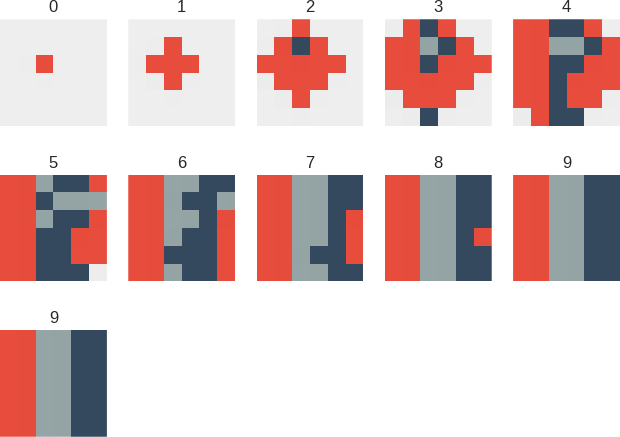
\includegraphics[height=0.4\textheight, width=\textwidth, keepaspectratio]{fig/result_figs/generate_tricolor/1}
\caption[A solution to the "Tricolor" morphogenesis]{A solution to the "Tricolor" morphogenesis that finds a point attractor equal to the target pattern.
Most solutions seen did not stabilize like this, but instead found a variety of cycles.}
\label{fig:tricolor_point_attractor}
\end{figure}

\begin{figure}[h]
\centering
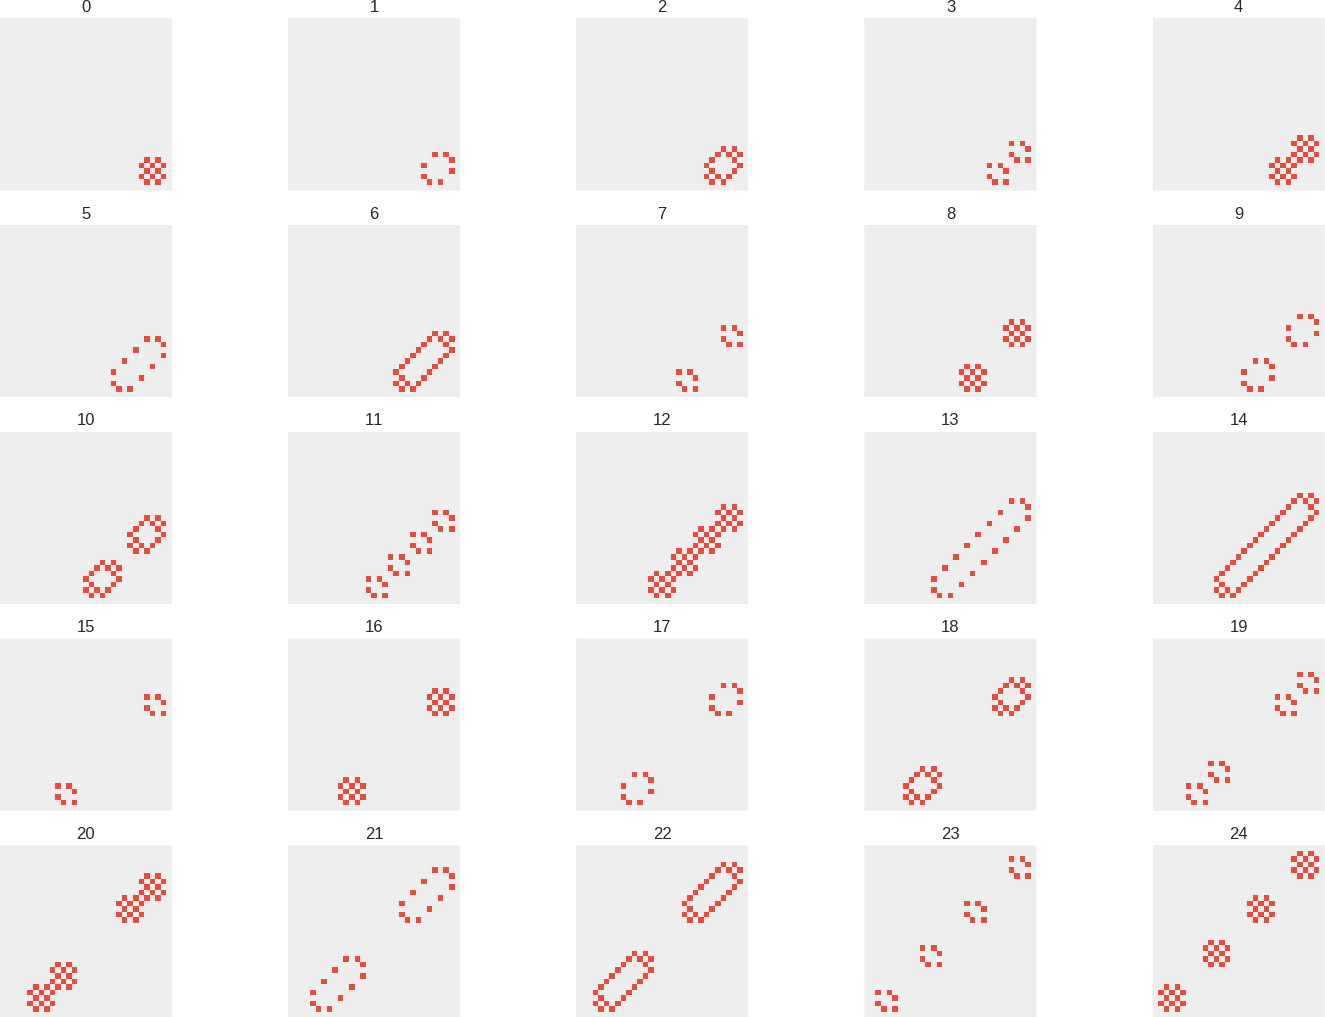
\includegraphics[height=0.4\textheight, width=\textwidth, keepaspectratio]{fig/result_figs/replicate_mosaic/7}
\caption[A solution to the "Mosaic" replication]{A solution to the "Mosaic" replication that shows multiple stages of replication.
First the original replicates into two copies. Then each copy tries to replicate, but they interfere with each other and instead return to one copy each, but at a greater distance.
Then they each succeed in replicating, producing four copies total.}
\label{fig:mosaic7}
\end{figure}


